\documentclass[]{article}

\usepackage{color, colortbl}
\usepackage{float}
\usepackage{graphicx}
\usepackage{listings}
\usepackage{multirow}
\usepackage{tabularx}
\usepackage{textcomp}

\usepackage[colorlinks]{hyperref}
\hypersetup{allcolors=blue}

\lstset{breaklines=true}

\newcommand{\tabitem}{~~\llap{-}~~}
\newcommand{\tabitemNum}{~~}

\definecolor{red}{rgb}{1,0.9,0.9}
\definecolor{green}{rgb}{0.9,1,0.9}


\title{Technical Design Report \\
	\large Software for Science - CERN Load Balancing}

\author{\textbf{Team 6 Hexoxide} \\
	Eloy Maduro Clement \\
	Geoffrey van Driessel \\
	Corne Lukken \\
	Bram Tukker}

\date{\textbf{\today} \\
	v1.0}


\begin{document}


\maketitle
\newpage


\section*{Introduction}
This document reflects the discovered \& analysed technical components for the CERN Load Balancing project. Components are identified in previously available documents as well as discoveries of the project team itself. 

Experiments and there setup are detailed so they can be repeated easily in the future as well as instructions how to install all required components. 


\section*{Changelog}
\begin{table}[H]
	\begin{center}	
		\begin{tabularx}{\textwidth}{ | l | l | X | }
			\hline
			\textbf{Version} & \textbf{Date} & \textbf{Description} \\ \hline
			
			\multirow{1}{*}{0.2} & 07-11-2018 & \tabitemNum 1. Added information on changing to debian image. \\
			& & \tabitemNum 2. Added information about investigating metric-beats for information logging. \\
			& & \tabitemNum 3. Added table of contents. \\
			& & \tabitemNum 4. Added information on how legacy software was setup and used. \\
			& & \tabitemNum 5. Added previously logged metrics and desired metrics. \\ \hline
			
			\multirow{1}{*}{0.3} & 01-12-2018 & \tabitemNum 1. Remove outdated or incoherent information. \\
			& & \tabitemNum 2. Add networking benchmarks. \\ \hline
			
			\multirow{1}{*}{0.4} & 07-12-2018 & \tabitemNum 1. Add installation instructions to report. \\
			& & \tabitemNum 2. Explain 94Mbit synthetic throughput. \\
			& & \tabitemNum 3. Introduction to alternative technologies. \\
			& & \tabitemNum 4. Incorporate research design into TDR. \\
			& & \tabitemNum 5. Add experiment network-baseline details. \\ \hline
			
			\multirow{1}{*}{0.5} & 12-12-2018 & \tabitemNum 1. Add operation diagram for network baseline experiment. \\
			& & \tabitemNum 2. Finish documentation of network baseline experiment. \\ \hline
			
			\multirow{1}{*}{0.6} & 10-01-2019 & \tabitemNum 1. Add round robin icn experiment. \\ \hline
			
			\multirow{1}{*}{0.7} & 15-01-2019 & \tabitemNum 1. Add source code documentation section. \\
			& & \tabitemNum 2. Add results for round robin ICN. \\ \hline
			
			\multirow{1}{*}{1.0} & 16-01-2019 & \tabitemNum 1. Determined mandatory changes. \\
			& & \tabitemNum 2. Improved hardware \& software setup introduction. \\
			& & \tabitemNum 3. Added networking diagrams. \\
			& & \tabitemNum 4. Described software and system components. \\
			& & \tabitemNum 5. Generalized SSH description. \\
			& & \tabitemNum 6. Described metricbeat and it’s metrics. \\
			& & \tabitemNum 7. Explained table underlinement. \\
			& & \tabitemNum 8. Describe the run operation for the round robin ICN experiment. \\
			& & \tabitemNum 9. Discussion \& results. \\
			& & \tabitemNum 10. MELK-installation-guide reference added \\
			& & \tabitemNum 11. MELK Sub Question. \\
			& & \tabitemNum 12. Added Zookeeper section. \\ \hline
		\end{tabularx}
	\end{center}
\end{table}
\newpage


\tableofcontents{}
\newpage


\section{Legacy software}
\textit{\textbf{Disclaimer: The legacy software has never reached an operational stage in the duration of Software for Science Load Balancing project 2018/2019 and although it provides details which will help others come a long way, it will take further steps to be able to use the legacy software to run experiments.}}

At the start of this project numerous previous experiments have been done on this subject. These previous experiments have led to the creation of existing software. It is important to identify how these softwares worked and references them so that they can be used in the future.

To make sure the exact version of the software can be retrieved the git version commit hashes are listed. To checkout a specific commit hash from a repository execute “git checkout COMMIT-HASH”.

\begin{table}[H]
	\begin{center}	
		\begin{tabularx}{\textwidth}{ | l | X | l | l | }
			\hline
			\textbf{Software} & \textbf{Purpose} & \textbf{Reference} & \textbf{Commit} \\ \hline
			
			O2Balancer & Binaries used in experiments containing specific algorithms to be tested. & \hyperref[sec:ref01]{O2 [1]} & 36eec89 \\ \hline
			
			BalancerScripts & Setting up nodes with ansible and orchestrating an experiment. Gathering and purging log files and creating plots and graphs from log data. & \hyperref[sec:ref02]{Scripts [2]} & 99f7177 \\ \hline
		\end{tabularx}
		\caption{Legacy Software.}
		\label{tab:specs}
	\end{center}
\end{table}

Newer software will likely still be distributed through git, but will be made available through the software-for-science github organisation. The repositories from previous experiments can now be on the organisation project. See this link for the page: \url{https://github.com/SoftwareForScience/O2-Balancer}


\section{Installation}
Documentation for the O2Balancer was based upon CentOS, as a result it might be difficult to get the software running for other types of Linux distributions although it has been successfully before. The documentation on how to install \& run the O2Balancer for the raspbian Linux distribution has been lost unfortunately. The installation instructions for CentOS can be found online on: \url{https://github.com/SoftwareForScience/O2-Balancer/blob/master/Docs/Compilation.md}

For other distributions with different package managers it should be fairly easy to replace the packages specified for the YUM package manager, however, installing all requirements for the O2Balancer can require a significant amount of system memory (between 8-16 gigabytes).

\subsection{Verify software installation}
Once the O2Balancer and its dependencies are installed, the installation can be verified by executing execute.sh in the build directory of O2Balancer, however, first zookeeper needs to be started.

\begin{lstlisting}
sudo /usr/share/zookeeper/bin/zkServer.sh start
./execute.sh
\end{lstlisting}

\subsection{Configuration arguments \& yaml files}
Each individual binary has command line arguments and a configuration file, some of the parameters configured through these two methods might override one or another.

\begin{table}[H]
	\textbf{InformationNode}	
	\begin{center}	
		\begin{tabularx}{\textwidth}{ | l | l | X | }
			\hline
			\textbf{Parameter} & \textbf{Data type} & \textbf{Description} \\ \hline
					
			--info-config & string & Path to yaml configuration file. \\ \hline			
			--sample-size & int & Size of individual packets send between FLP \& EPN in MB. \\ \hline
			--ip & string & ? \\ \hline
		\end{tabularx}
		\caption{ICN parameters.}
		\label{tab:specs}
	\end{center}
\end{table}

\begin{table}[H]
	\textbf{FLP}	
	\begin{center}	
		\begin{tabularx}{\textwidth}{ | l | l | X | }
			\hline
			\textbf{Parameter} & \textbf{Data type} & \textbf{Description} \\ \hline	
					
			--flp-config & string & Path to yaml configuration file. \\ \hline			
			--restartFairRoot & boolean & ? \\ \hline
			--ip & string & ? \\ \hline
		\end{tabularx}
		\caption{FLP parameters.}
		\label{tab:specs}
	\end{center}
\end{table}

\begin{table}[H]
	\textbf{EPN}	
	\begin{center}	
		\begin{tabularx}{\textwidth}{ | l | l | X | }
			\hline
			\textbf{Parameter} & \textbf{Data type} & \textbf{Description} \\ \hline	
					
			--epn-config & string & Path to yaml configuration file. \\ \hline
			--amount-flps & int & Amount of FLP’s in this experiment the EPN will expect data from. \\ \hline
			--flp-port & int & The network port the EPN will listen on for data from the FLP. \\ \hline
			--ip & string & ? \\ \hline
		\end{tabularx}
		\caption{EPN parameters.}
		\label{tab:specs}
	\end{center}
\end{table}

The execute.sh script will open a total of 6 windows which should appear, each running a different type of node software. In total there should be 3 EPN’s, 2 FLP’s \& 1 InformationNode.


\section{Hardware Specifications}
According to the A Large Ion Collider Experiment (ALICE) technical design report \hyperref[sec:ref01]{TDR [1]}, there will be two types of computing nodes in the O2 project after long shutdown 2 (LS2). In total there will be about 2000 nodes in O2, 250 so called FLP nodes and 1750 EPN nodes.

A set of 80 computing devices grouped in units of four has been provided by the Amsterdam University of Applied Sciences (AUAS) for this project. These 80 nodes will be used to simulate network scenarios as close as possible to the actual O2 computing network. The computing devices at AUAS will be Raspberry Pi’s, specifically, model 3 B+.

In table 1 a comparison of differences in hardware is detailed. It is clear that the computing nodes provided by AUAS are vastly inferior to the computing hardware that will become available for ALICE O2. These hardware differences must be taken greatly into account during the project and its various experiments.

\begin{table}[H]
	\begin{center}
		\begin{tabular}{ | l | l | l | l | }
			\hline
			\textbf{Component} & \textbf{FLP (250)} & \textbf{EPN (1750)} & \textbf{Raspberry Pi 3 B+ (80)} \\ \hline
			
			CPU & ? x86 & 32 Core x86 & 4 Core ARMv8 \\ \hline
			RAM & 32GB & 128GB & 1GB \\ \hline
			Ethernet & 4 x 10Gbit & 10Gbit & 300Mbit \\ \hline
		\end{tabular}
		\caption{Hardware specifications of computing nodes.}
		\label{tab:specs}
	\end{center}
\end{table}


\section{Synthetic benchmarks}
To measure the maximum throughput that can be achieved on the network the \hyperref[sec:ref04]{iPerf3 [4]} tool was used to measure the throughput for 10 seconds. The measurement was repeated 50 times. The results show that the network throughput has a relatively low variance and is almost always consistently 94Mbit/s.

This 94Mbit of throughput even though the Raspberry Pi has a 1Gbit interface limited to 300Mbit due to sharing an USB 2.0 host controller was expected. This limited throughput is due to the Raspberry Pi’s being connected via a 100Mbit switch.

\begin{center}
	\begin{figure}[H]
		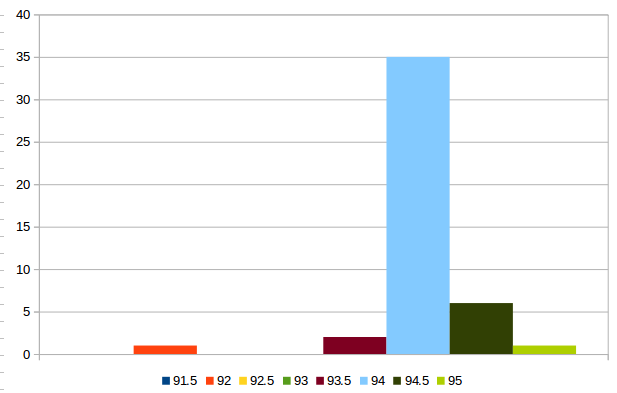
\includegraphics[width=\textwidth]{images/network-benchmark}
		\caption{Distribution of synthetic benchmark throughput.}
		\label{fig:ssh}
	\end{figure}
\end{center}


\section{Hardware \& software setup}
The pi clusters used in experiments were initially empty. So the pi clusters are configured with an image. To speed up the initial process, one image was made and reused for the other clusters. The required dependencies were also installed on the initial image. A bash script was developed which helps with the installation of the dependencies. The remaining processes were automated with Ansible. All the scripts to speed up initial pi cluster setup are stored in repository that are publicly accessible and listed within this document.

Raspberry pi nodes are ARM based and this can pose limits on the available software, for instance Logstash will not compile or run on ARM based systems. It is important to take these limits into account and before starting to implement properly investigate software and its availability.

\subsection{Network}
The network during the experiments consisted of 8 raspberry-pi nodes each with two network interfaces. One of these interface had an internet connection through a bridged router but was segregated from the actual internal network using Network Address Translation (NAT). The initial system design has every component installed on one raspberry pi but unfortunately some system components turned out to be incompatible with ARM based processors. An virtual machine running on an X86 based host was configured to resolve any ARM related issues, however, this host resided outside the NAT segregated network and additional steps using port forwarding and additional NAT were required to resolve them.

The following networking diagram shows an overview of the entire network using Cisco diagramming standards. In this diagram the host at 192.168.3.2 is the virtual machine responsible for running X86 system components while the host at 192.168.3.4 is the router responsible for segregating the raspberry-pi’s from the rest of the internal network. Each of the firewalls indicate the NAT that occurs on two places in the network and this will require port forwarding and tunneling later.

\begin{center}
	\begin{figure}[H]
		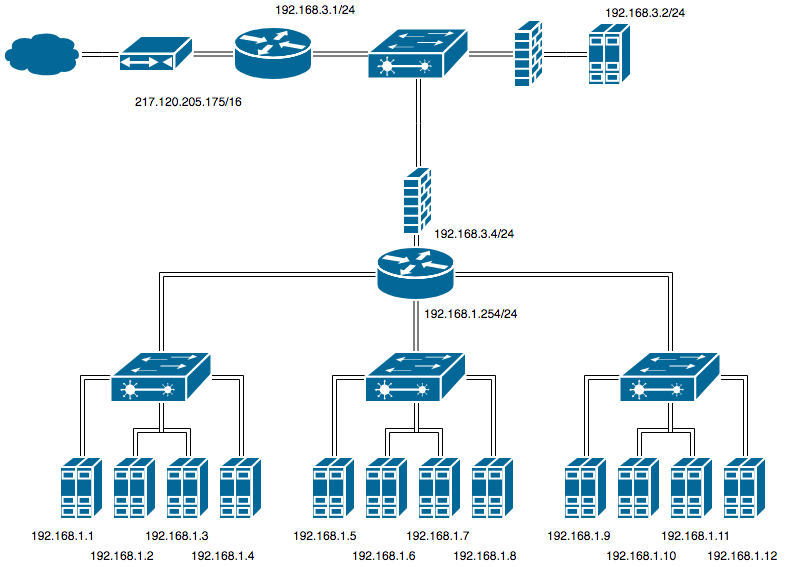
\includegraphics[width=\textwidth]{images/network-primary}
		\caption{Networking diagram with auxiliary networking interfaces omitted. A diagram with the auxiliary interface can be found \hyperref[sec:ref05]{online [5]}.}
		\label{fig:ssh}
	\end{figure}
\end{center}

\subsection{New software introduction}
An environment as similar as possible to the one used at CERN is desired, however, it has proven to be not feasible to use CentOS. This is due to the limitations the Raspberry pi version has in comparison to the CentOS x86\_64 image. One of the main reasons is the inability to switch of gcc version, normally, a tool called scl provides the switching for specific versions of many development tools. The version of gcc supplied with CentOS is incompatible with the version of boost that is specified in many of the previous experiments. Furthermore the version of gcc is not capable of compiling c++2011 features which is required by CERN. To continue to use CentOS gcc would have to be built to be build from source.

To resolve the issues with the CernOS image an alternative had to be elected. Based on previous experience Manjaro 17.1 was chosen, Manjaro provides a full features ARM image for which a tremendous amount of packages are available. Manjaro being an Arch based distribution is extremely permissive in adaptive configurations allowing it to closely reflect any other distribution.

Unfortunately due to the rolling release model of Manjaro even this eventually led to great trouble, which included: Broken packages, unavailable mirrors and missing kernel modules. As an alternative Raspbian stretch was chosen because of its tremendous support and large community which should allow to more easily mitigate problems.

Based on the reports of the previous experiments a table could be compiled which compares the version of libraries from the legacy software to the versions used in the new software. It should be noted that the information about the legacy software was determined to be partially incorrect as it does not use FairMQ itself but instead relies on FairRoot.

\begin{table}[H]
	\begin{center}
		\begin{tabular}{ | l | l | l | }
			\hline			
			\textbf{Library/Tool} & \textbf{Version used} & \textbf{Version Legacy Software} \\ \hline
			
			FairMQ & 1.3.6 & 1.1.5 \\ \hline
			ZeroMQ & 4.2.5 & 4.2.1 \\ \hline
			Zookeeper & 3.4.9 & 3.4.9 \\ \hline
			Cmake & 3.12.4 & 3.11.0 \\ \hline
			Boost & 1.66.0 & 1.66.0 \\ \hline
			Yaml-cpp & NONE & 0.5.2 \\ \hline
			FairLogger & 1.3.0 & NONE \\ \hline
			Compiler & gcc 6.3.0 & gcc 6.3.0 \\	\hline
		\end{tabular}
		\caption{The installed software dependencies on the pi’s.}
		\label{tab:librabies}
	\end{center}
\end{table}

\subsection{New software \& system components}
The system consist of different nodes all of which are running Debian as operating system and which are accessible using SSH. The Raspberry pi based nodes have all dependencies installed using the raspberry-dependency repository and its install scripts. The X86 based virtual machine has different software components installed which will be described later for these components an installation guide is available in the documentation repository.

\begin{table}[H]
	\begin{center}
		\begin{tabularx}{\textwidth}{ | l | X | }
			\hline			
			\textbf{Repository} & \textbf{Purpose} \\ \hline
			
			\hyperref[sec:ref06]{raspberry-dependency [6]} & Detailed instructions listing required Debian packages and automated install script to install further dependencies not installed through package manager. \\ \hline
			\hyperref[sec:ref07]{BalancerScripts2 [7]} & Small scripts that can be executed from the command line to orchestrate and/or configure software components that allow the experiment to run across different nodes. \\ \hline
			\hyperref[sec:ref08]{O2-Balancer2 [8]} & Core binaries which run the experiments by configuring and sending data on different channels across the network. \\ \hline
			\hyperref[sec:ref09]{Documentation [9]} & Essential documentation on the overall project as well as how to get started with the continuation of our project. \\ \hline
		\end{tabularx}
		\caption{Overview of essential repositories.}
		\label{tab:librabies}
	\end{center}
\end{table}

\subsection{Installation}
To ensure the reproducibility of experiments executed by the new software, a \hyperref[sec:ref06]{bash script [6]} has been developed which will install all the dependencies automatically. The installation instructions are based on Debian distributions and additional effort could be required to be able to use them on different distributions. Along this installation scripts additional documentation is available in the documentation repository which will allow to configure the X86 based system components.

\subsection{SSH}
Remote access to each of the individual nodes is done via SSH in the setup the first node is used a portal to access the other nodes in the network. Using a single node as portal limits the amount of ports that needs to be forwarded to the outside network. Additionally an SSH key from the portal node can be added to every node so that SSH logins no longer require a username \& password after logging into the portal.

The SSH configuration also uses ssh tunneling this is done to allow access to an web based dashboard running on the X86 based virtual machine.

\begin{center}
	\begin{figure}[H]
		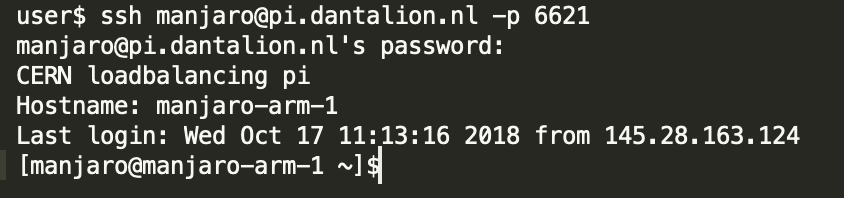
\includegraphics[width=\textwidth]{images/ssh}
		\caption{Example of login in using SSH on remote accessible raspberry pi.}
		\label{fig:ssh}
	\end{figure}
\end{center}

\subsection{Ansible}
To run and configure tests on the pi clusters, some things will need to be configured. Ansible will be used to handle the configuration of each pi, defining which experiments to run and with which parameters to do so. Ansible allows to apply different parameters to different categories of hosts.

\subsection{MELK}
Metricbeat can be used to gather statistics of the nodes. This data can be send to Logstash, which should have run on the ICN. Then, Logstash can output the data in two ways:
\begin{itemize}
	\itemsep 0em
	\item Plain text file
	\item Elasticsearch
\end{itemize}

To easily visualize the data, Kibana can be used to retrieve the data from Elasticsearch. This service should also run on the icn. By port forwarding the service on an external machine, Kibana can be viewed inside a web browser.

Due to incompatibilities with Logstash on ARM both Logstash and ElasticSearch were installed on the X86 virtual machine. The overall experience with MELK was very poor the exact problems, discoveries and conclusion will be discussed later.

Kibana is part of the ELK stack, which is used to properly interpret metrics from the hardware and network during experiments. ELK is short for Elasticsearch, Logstash and Kibana. These three pieces of software process incoming data from hardware components running Metricbeat.

\subsubsection{Elasticsearch}
Elasticsearch is a distributed, RESTful search and analytics engine capable of solving a growing number of use cases. As the heart of the Elastic Stack, it centrally stores the data.

\subsubsection{Logstash}
Logstash is an open source, server-side data processing pipeline that ingests data from a multitude of sources simultaneously, transforms it, and then sends it to Elasticsearch.

\subsubsection{Kibana}
Kibana is able to visualize Elasticsearch data and navigate the Elastic Stack, and can do so using a wide range of visualizations.

\subsubsection{Metricbeat}
Collect metrics from systems and services. From CPU to memory, Redis to NGINX, and much more, Metricbeat is a lightweight way to send system and service statistics. However, in the setup for running O2-Balancer experiments, the data gathered is limited to metrics such as CPU load (in percentages), memory usage (in MegaBytes), and network throughput (in KiloBytes per second).

\subsubsection{Data}
While Metricbeat offers a wide range of data to send, in the setup for running O2-Balancer experiments, the data gathered is limited to metrics such as:
\begin{itemize}
	\itemsep 0em
	\item CPU load (in percentages)
	\item Memory usage (in MegaBytes)
	\item Network throughput (in KiloBytes per second)
	\item Network latency (in milliseconds)
\end{itemize}

\subsubsection{Visualizations}
Kibana offers several types of visualizations: charts such as area, heat map, horizontal and vertical bar and pie. For the purpose of the experiments and their effects on the hardware and network, line charts proved to be most effective in visualising the relevant data, because these showed changes over time.
These graphs are then displayed in a grid formation on a dashboard, which created an ordered overview of all measured statistics.

\begin{center}
	\begin{figure}[H]
		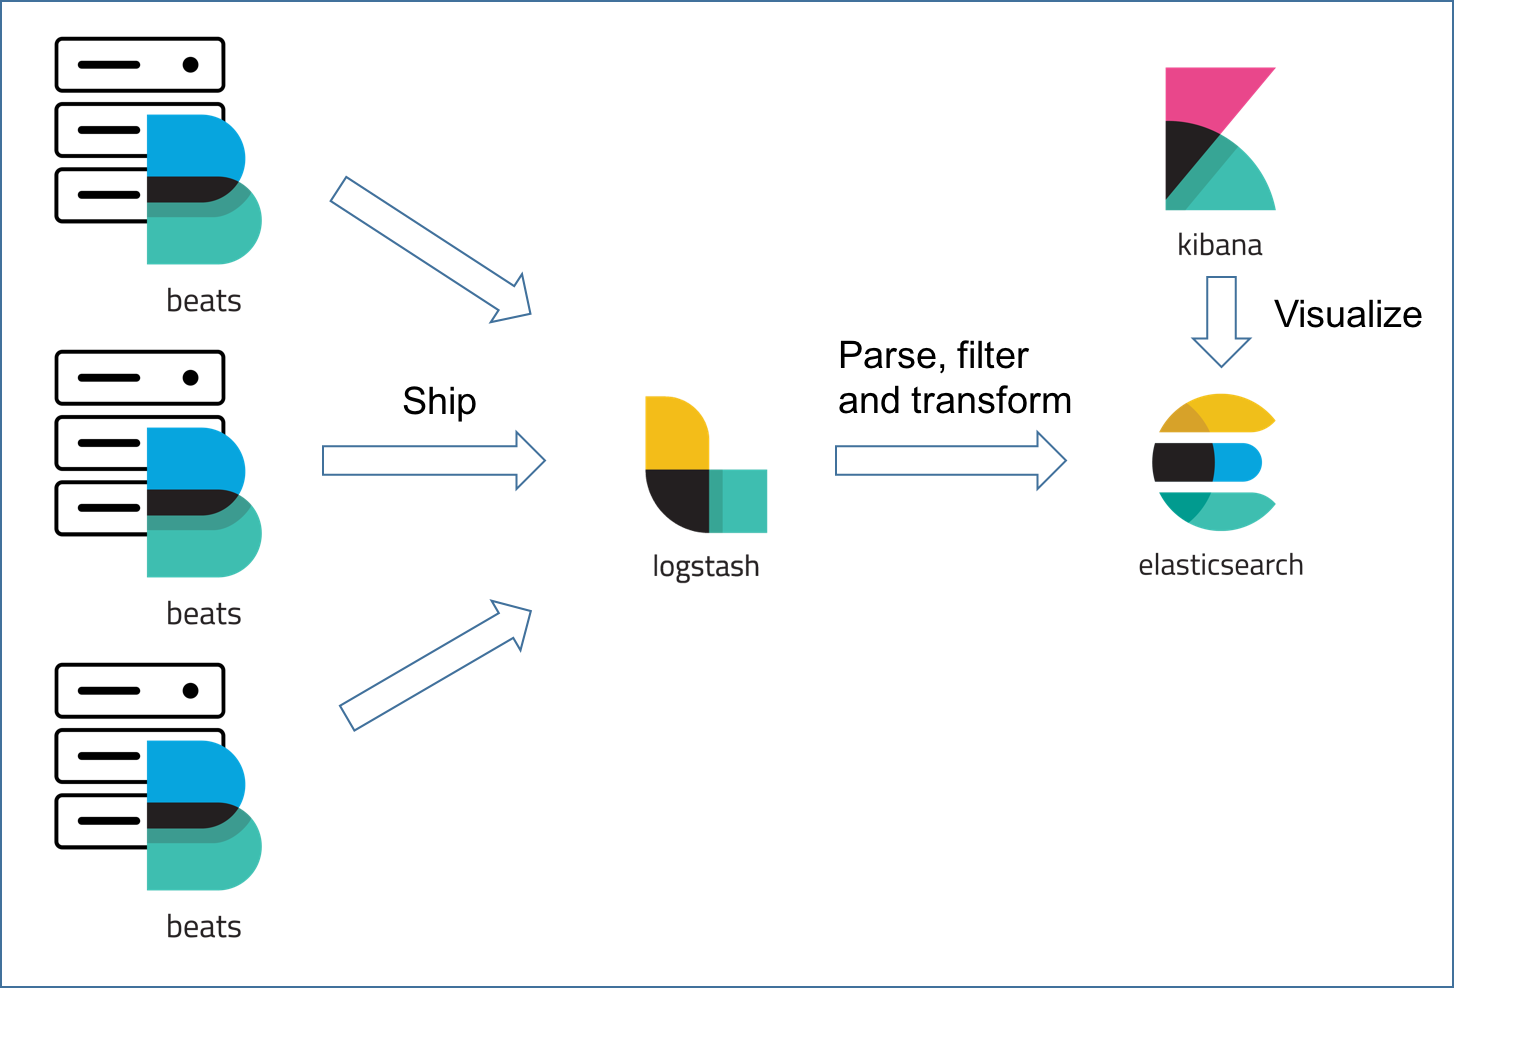
\includegraphics[width=\textwidth]{images/melk}
		\caption{Overview of MELK stack.}
		\label{fig:ssh}
	\end{figure}
\end{center}

\subsubsection{Logging metrics}
The decision to use Metricbeat was heavily based on it’s extensive selection of different metrics. The following overview of metrics shows what was intended to be used to evaluate different experiments.

\begin{table}[H]
	\begin{center}
		\begin{tabular}{ | c | c | c | }
			\hline
			\textbf{\#} & \textbf{Metric} & \textbf{Measure} \\ \hline
			
			1 & Temperatures & degrees Celsius ($^\circ$C) \\ \hline
			2 & Throughput & KiloBytes per second (KB/s) \\ \hline
			3 & Scaling governer / Core clock & MegaHertz (MHz) \\ \hline
			4 & Memory usage & MegaBytes (MB) \\ \hline
			5 & CPU usage & Percentage (\%) \\ \hline
			6 & Swap & MegaBytes (MB) \\ \hline
			7 & Fail-over & Number of Nodes (NoN)\\ \hline
		\end{tabular}
		\caption{Metric that will be used in the experiments.}
		\label{tab:specs}
	\end{center}
\end{table}


\section{Source Code Documentation}
Beside the regular documentation, the source code itself can also be documented. This helps understanding what the code does. This especially important for the developers, since they might have to modify the logic or add additional features.

This project uses Doxygen to create the documentation. Doxygen is a library that can automatically generate documentation by scanning through the source file for specific comments.Furthermore, Doxygen can extract the file structure of the project. The output will be in the form of a HTML webpage or multiple LaTeX files. 

\subsection{Generate}
In order to use Doxygen for this project, it should be installed on the machine beforehand. It’s important to note that Doxygen will be executed through CMake. So the path to the library should be finable for CMake.

Normally, the documentation will be automatically generated when building the project. However, this can be disabled through the following command:
\begin{lstlisting}
cmake -DENABLE_DOXY=OFF
\end{lstlisting}

\subsection{Access}
After Doxygen has been executed, the documentation can be found in the ‘docs’ directory, located in the root directory of the project.

To access the html version, open ‘index.html’ inside a web browser. The file is location in the ‘html’ directory. Here follows a overview of the most important sections:
\begin{itemize}
	\itemsep 0em
	\item \textbf{Main Page}: Contains the REAME.md file of the project.
	\item \textbf{Classes \textrangle{} Class List}: Shows a list of all the classes.
	\item \textbf{Classes \textrangle{} Class Members}: Shows a list of all the functions and variables of the classes.
	\item \textbf{Files \textrangle{} File List}: Overview of the project structure.
\end{itemize}

\subsection{Modify}
There are several ways to put comment in the source code. Here follows the template comments used in this project.
\begin{itemize}
\item \textbf{Block}
\begin{lstlisting}
/*
* [description]
* [more description]
*/
[entity]
\end{lstlisting}

\item \textbf{Brief description (for classes)}
\begin{lstlisting}
/// [description]
[entity]
\end{lstlisting}

\item \textbf{One line}
\begin{lstlisting}
/** [description] */
[entity]
\end{lstlisting}

\item \textbf{After member}
\begin{lstlisting}
[member] /**< [description] */
\end{lstlisting}

\end{itemize}

For the full documentation of Doxygen on this topic, please see: \url{http://www.doxygen.nl/manual/docblocks.html}


\section{Research design}
The research design describes the approach of the experiments.

\subsection{Problem Statement}
Before diving into the research, this paragraph describes the general problem of the research.The problem is a specific problem of CERN, but the research itself should be applicable across other similar problems.

\subsubsection{ALICE}
ALICE, which stands for A Large Ion Collider Experiment, is one of many detectors mounted on the Large Hadron Collider (LHC) at CERN. ALICE is used to study states of matter in extreme energy densities. Specifically, a state of matter known as quark-gluon plasma. This state is achieved by shooting two lead ions against each other inside the LHC. This results in temperatures over 100,000 times the center of the sun.

\subsubsection{Problem}
ALICE will be upgraded their systems during the Long Shutdown 2 (LS2). This upgrade will significantly increase the data gathered. It is estimated that the collection of data will increase by a factor of 100, which roughly translates to 1.1 TB/s of continuous throughput.

This upgrade also comes with an upgrade of the computing infrastructure capable of handling the increase in data collection; i.e. increasing and improving the amount of First Level Processors (FLPs) and Event Processing Nodes (EPNs), as well as the networking infrastructure. The computing upgrade will need to be accompanied by software to efficiently handle load balancing.

\subsection{Research Framework}
The research framework below shows the resources (existing research, et cetera) used to construct the conceptual model with which the objects of research (Sub-TimeFrames, Fair MQ, et cetera) were put to the test. Results of those test were finally gathered and used to make recommendations.

\begin{center}
	\begin{figure}[H]
		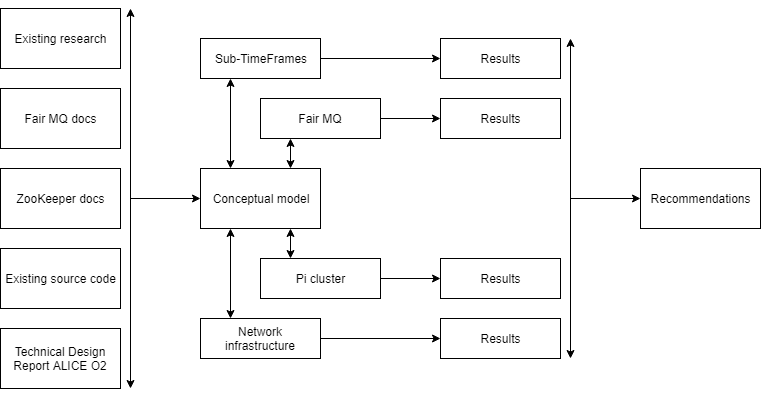
\includegraphics[width=\textwidth]{images/research-model}
		\caption{A Schematic representation of the research (focussed on the actual experiments).}
		\label{fig:ssh}
	\end{figure}
\end{center}

\subsection{Main Research Question}
Based on the problem statement and the research framework, a main research question can be established. The focus is on trying new approaches for the load balancer, with the goal of improving the overall performance and usability. A comparison will be made between these approaches to give an overview of the advantages and disadvantages. That’s why the main research question is defined as follows: \textit{“How do different load-balancing algorithms compare in transferring a continuous data stream across parallel many-to-one streams?”}

\subsection{Sub Research Question}
In order to answer the main research question, a few sub question are established to divide the whole research into smaller parts. This will be handy, especially for the different algorithms that will be used for each approach. These are the sub questions:
\begin{itemize}
	\itemsep 0em
	\item Which algorithms have been developed already and what are the results?
	\item What are potential alternatives on which experiments can be run?
	\item Which metrics are available to the validate the quality of the experiments?
	\item How can the metrics be visualised using Kibana?
\end{itemize}


\section{Experiments}
Experiments are documented in 4 parts starting with a general introduction / description. After that the configuration is detailed and the necessary information is provided to revalidate the experiment. An operational overview and description is given and finally the results are measured. The experiments will only detail preliminary results and a conclusive total overview of results and how they evaluate together can be found in the results chapter. 

The necessary information to revalidate an experiment can be found by using the references in the configuration section.

In the tables describing the experiments the specific results which have the same throughput as the maximum determined in the synthetic benchmark will be underlined. The following short table is an example of that underlining.

\begin{table}[H]
	\textbf{Example for underlining synthetic benchmark equivalent throughput}
	\begin{center}
		\begin{tabular}{ | l | l | l | }
			\hline
			\textbf{Rate (Hertz)} & \textbf{Message size (Bytes)} & \textbf{Percentage loss (\%)} \\ \hline
			
			200 & 58000 & 0.00 \\ \hline
			\underline{200} & \underline{58750} & \underline{0.49} \\ \hline
		\end{tabular}
		\caption{Underlining of the synthetic benchmark equivalent allows for quickly comparing results.}
		\label{tab:specs}
	\end{center}
\end{table}

\subsection{Network throughput baseline}
This experiments tests network throughput using the FairMQ application layers after having measured the maximum throughput that could be achieved on the specific hardware using the synthetic benchmark. The absolute maximum throughput that can be achieved is 94Mbit as demonstrated with iperf3.

The 94 Mbit throughput can be translated into a 11.75 Mbyte throughput. With the message rate of 200Hz it can be determined that the network should be able to sustain a message size of 58750 bytes. The number of FLP’s and the message size was varied during this experiment.

The experiment should run for 30 seconds and is validated with tight timing constraints, the total experiment time should be no less than 29.7 seconds and no more than 30.3. Failure of a run to be within these timing constraints means it will not be used as part of the results.

\subsubsection{Configuration}

\begin{table}[H]
	\begin{center}
		\begin{tabular}{ | l | l | l | l |}
			\hline
			Rate & 200Hz & \multicolumn{2}{ c | }{\textbf{Node}} \\ \hline
			
			Messages & 6000 & \textbf{Type} & \textbf{Ip} \\ \hline
			Runtime & 30 seconds & ICN & 192.168.1.4 \\ \hline
			Message size & Variable & FLP 1 & 192.168.1.3 \\ \hline
			Source commit & \hyperref[sec:ref10]{cbaebb9 [10]} & EPN & 192.168.1.2 \\ \hline
			Documentation &  \hyperref[sec:ref11]{cdbb643 [11]} & FLP 2 & 192.168.1.5 \\ \hline
			Arguments & \hyperref[sec:appendix01]{appendix} & FLP 3 & 192.168.1.6 \\ \hline
		\end{tabular}
		\caption{The specific configuration lists essential parameters as well as the specific commit referencing to the source code.}
		\label{tab:specs}
	\end{center}
\end{table}

The experiment consisted of 9 different configurations were both the message size and the number of FLP’s in the network were varied. Each configuration was run for 30 times so additional statistical analysis could be performed if required.

\subsubsection{Operation}
The operation of the experiment involved a two step procedure, were in the first step the binaries are configured and in the second step the actual experiment is run. During this experiment the ICN it’s available channels are hardcoded into the binary and could only be changed at compile time. 

The three different core Binaries are started at the same time and the EPN \& FLP will wait for incoming messages while the ICN starts counting down a 10 second wait period. After the grace period the ICN will send the EPN channel configuration to all FLP’s. After the message has been send the ICN will wait an additional 2 seconds for the FLP’s to configure the newly received channels. When the ICN has waited for the FLP’s to be configured the experiment will run.

\begin{center}
	\begin{figure}[H]
		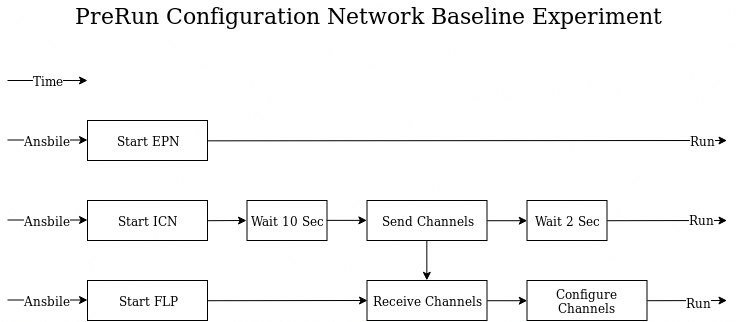
\includegraphics[width=\textwidth]{images/no-zookeeper-flow-n-base-exp}
		\caption{PreRun configuration stage depicts different operations across each type of node in time.}
		\label{fig:ssh}
	\end{figure}
\end{center}

The network is shown for each of the possible configurations during the experiment which indicates the physical location of each node in the network. All connections between devices are 100Mbit.

\begin{table}[H]
	\textbf{Network setup}
	\begin{center}
		\begin{tabular}{ | c | c | c | }
			\hline
			\textbf{1 FLP} & \textbf{2 FLP} & \textbf{3 FLP} \\ \hline
			
			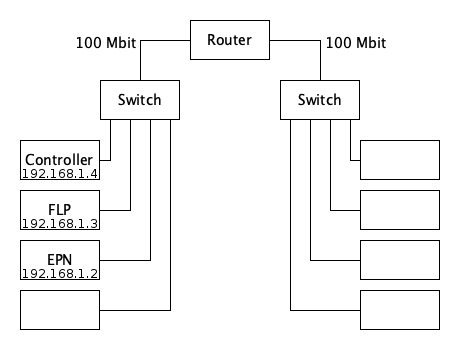
\includegraphics[width=0.3\textwidth]{images/network-baseline-1} & 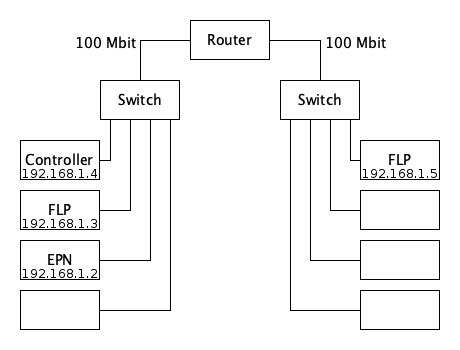
\includegraphics[width=0.3\textwidth]{images/network-baseline-2} & 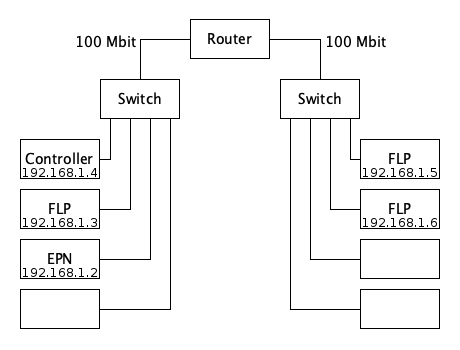
\includegraphics[width=0.3\textwidth]{images/network-baseline-3} \\ \hline
		\end{tabular}
		\caption{Network diagrams for each number of FLP configurations.}
		\label{tab:specs}
	\end{center}
\end{table}

\subsubsection{Results}
During the synthetic benchmarks the maximum network bandwidth was determined to be 94Mbit. In accordance to this synthetic throughput a maximum message size of 58750 bytes and 1 FLP is expected to have close to zero or zero loss. In a similar fashion a message size of 29375 bytes with 2 FLP’s was expected to have similar loss. 

During the experiment it became clear that having multiple FLP’s further limits the amount of available bandwidth available for throughput between FLP’s and EPN’s. Attempting to sustain a throughput of 93 Mbits with more than one FLP results in significant loss of messages, furthermore, increasing the message size beyond the equivalent of 93 Mbit throughput also results in significant loss of messages. 93 Mbit is close but not equivalent of 94 Mbit this lower throughput is likely due to the network traffic from ICN to FLP \& from EPN to ICN because these network connections aren’t present in the synthetic benchmark.

The results shows that the number of FLP’s has an impact on the maximum throughput that can be achieved and that this should be taken into account in further experiments. 

\begin{table}[H]
	\textbf{Mean message loss per configuration - 6000 messages sent}
	\begin{center}
		\begin{tabularx}{\textwidth}{ | X | X | X | X | }
			\hline
			\textbf{Number of FLP’s} & \textbf{Message size (per FLP)} & \textbf{Mean loss (total)} & \textbf{Mean loss (\%)} \\ \hline
			
			1 & 58000 & 2.333333333 & 0.03 \\ \hline
			\underline{1} & \underline{58750} & \underline{42.13333333} & \underline{0.70} \\ \hline
			1 & 59500 & 119.7333333 & 1.99 \\ \hline
			
			2 & 29000 & 148.3666667 & 2.47 \\ \hline
			\underline{2} & \underline{2937}5 & \underline{121.4333333} & \underline{2.02} \\ \hline
			2 & 29750 & 120.8666667 & 2.01 \\ \hline
			
			3 & 19333 & 196.1 & 3.26 \\ \hline
			\underline{3} & \underline{19583} & \underline{198.6333333} & \underline{3.31} \\ \hline
			3 & 19833 & 885.4333333 & 14.75 \\ \hline
		\end{tabularx}
		\caption{Message loss during the network baseline with 200Hz event rate.}
		\label{tab:specs}
	\end{center}
\end{table}

\subsection{Round Robin ICN}
This experiment tests the achievable throughput with minimal packet loss using the same algorithm as performed with previous version of the software. Each of the available EPN’s is selected in turn by incrementing an iterator and returning it to the start if the last element has been accessed. 

8 Node’s are configured during this experiment and the AliceO2 ratio of 1:6 with regards to the FLP and EPN’s is achieved. Both 50Hz and 200Hz event rates will be tested to completely cover the event operating range of the network after LS2.

Each configuration is ran for 10 iterations to achieve a normal distribution should advanced statistical analysis be required later. Additionally each configuration gets one iteration where the total operation time is set to 3 minutes instead of 30 seconds so that any variation caused by iteration time can be detected. This will also help determining if an iteration time of 30 seconds is sufficient as this has been used as iteration time in past experiments as well as these experiments. The rationale is that the short iterations could hide potential network bottlenecks that are mitigated using network buffers, however, network buffers can only mitigate such a network bottleneck for a short duration so, as a result the longer iteration time should discover these problems.

\begin{center}
	\begin{figure}[H]
		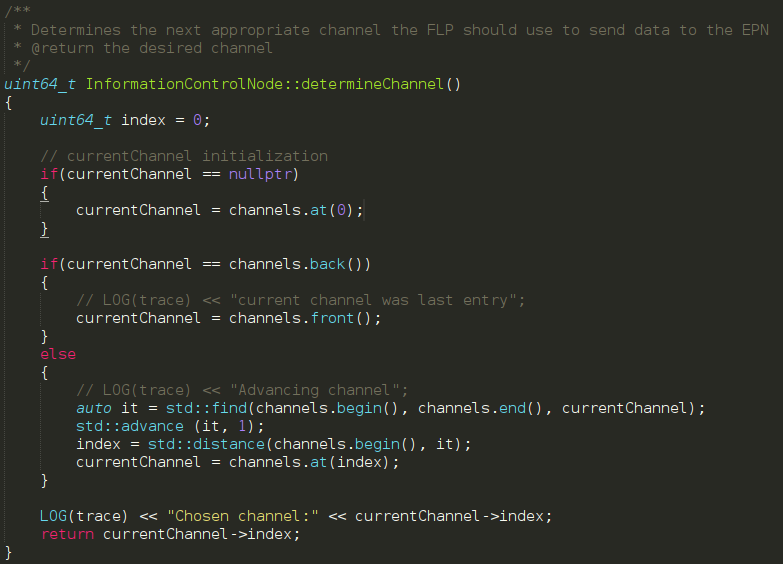
\includegraphics[width=\textwidth]{images/determine-channel}
		\caption{Channel determination for round robin.}
		\label{fig:ssh}
	\end{figure}
\end{center}

\subsubsection{Configuration}

\begin{table}[H]
	\begin{center}
		\begin{tabular}{ | l | l | l | l |}
			\hline
			Rate & 50Hz / 200Hz & \multicolumn{2}{ c | }{\textbf{Node}} \\ \hline
			
			Messages & 1500 / 6000 & \textbf{Type} & \textbf{Ip} \\ \hline
			Runtime & 30 seconds & ICN & 192.168.1.1 \\ \hline
			Message size & Variable & FLP 1 & 192.168.1.2 \\ \hline
			Source commit & \hyperref[sec:ref10]{5914f78 [10]} & EPN 1 / FLP 2 & 192.168.1.3 \\ \hline
			Documentation &  \hyperref[sec:ref11]{347173e [11]} & EPN 2 & 192.168.1.4 \\ \hline
			Arguments & \hyperref[sec:appendix02]{appendix} & EPN 3 & 192.168.1.5 \\ \hline
			\multicolumn{2}{ | l | }{\multirow{3}{*}{}} & EPN 4 & 192.168.1.6 \\
			\multicolumn{2}{ | l | }{} & EPN 5 & 192.168.1.7 \\
			\multicolumn{2}{ | l | }{} & EPN 6 & 192.168.1.8 \\ \hline
		\end{tabular}
		\caption{The specific configuration lists essential parameters as well as the specific commit referencing to the source code.}
		\label{tab:specs}
	\end{center}
\end{table}

A total of 14 different configurations were tested during this experiment. The message size, event rate and the amount of FLP’s in the network were varied. The differences between these configurations should demonstrate the effects on the effective bandwidth of the network with an event rate of 200Hz.

\begin{table}[H]
	\textbf{Configuration overview}	
	\begin{center}
		\begin{tabular}{ | l | l | l | l | }
			\hline
			\textbf{\#} & \textbf{Message size (Bytes)} & \textbf{Rate (Hertz)} & \textbf{Number of FLP’s} \\ \hline
			
			1 & 232000 & 50 & 1 \\ \hline
			\underline{2} & \underline{235000} & \underline{50} & \underline{1} \\ \hline
			3 & 238000 & 50 & 1 \\ \hline
			4 & 58000 & 200 & 1 \\ \hline
			\underline{5} & \underline{58750} & \underline{200} & \underline{1} \\ \hline
			6 & 59500 & 200 & 1 \\ \hline
			7 & 65000 & 200 & 1 \\ \hline
			8 & 116000 & 50 & 2 \\ \hline
			\underline{9} & \underline{117500} & \underline{50} & \underline{2} \\ \hline
			10 & 119000 & 50 & 2 \\ \hline
			11 & 29000 & 200 & 2 \\ \hline
			\underline{12} & \underline{29375} & \underline{200} & \underline{2} \\ \hline
			13 & 29750 & 200 & 2 \\ \hline
			14 & 32500 & 200 & 2 \\ \hline
		\end{tabular}
		\caption{All 14 configurations during the round robin ICN experiment.}
		\label{tab:specs}
	\end{center}
\end{table}

In the results section the configuration numbers will be reused as a method to uniquely identify configurations as a result it should easier to cross-reference and get a good overview of how configurations compare.

\subsubsection{Operation}
The operation is similar to the network baseline experiment but additional automatic configuration has been added to simplify the process. The overall operation still consist of a two step procedure but the EPN’s have additional features that allow them to report their listening channel to the ICN. This allows to ICN to maintain a list of EPN’s that are available which can then be iterated over in a round robin fashion.

During the PreRun step the EPN will wait ten seconds after being started and will then proceed by sending its channel data to the ICN. This initial delay allows ICN to be started without very tight timing constraints as delays between nodes could differ in a network. The ICN is configured to be dormant until it receives the first channel. After receiving the first channel it will allow for additional channels to be added during a ten second period. After this period it will forward all the channels to the FLP’s in the network and it will wait two seconds before continuing. During this two second period the FLP’s will have time to configure their channels. With the FLP their channels configured the PreRun step is finished and the run step is entered.

\begin{center}
	\begin{figure}[H]
		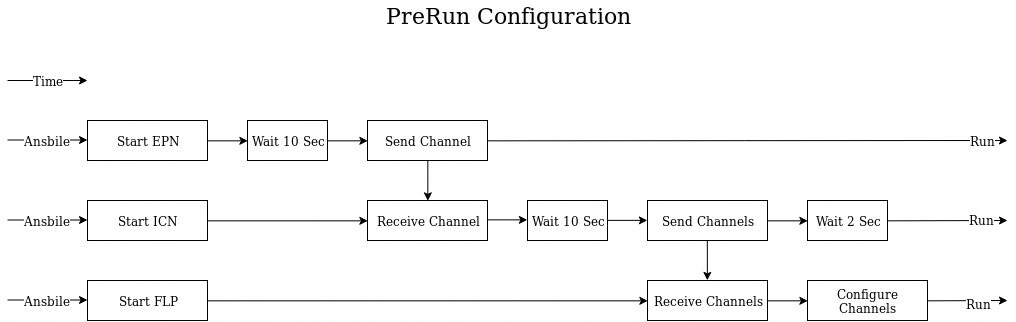
\includegraphics[width=\textwidth]{images/no-zookeeper-flow}
		\caption{PreRun configuration stage depicts different operations across each type of node in time.}
		\label{fig:ssh}
	\end{figure}
\end{center}

During the run step the ICN will monitor the rate of transmission. Whenever the FLP should send the next message to the currently selected EPN the ICN will send an message to the FLP. This message will contain an heartbeat ID as well as the selected EPN that should receive the message. The ICN will then increment the list of EPN’s as a means to select the next one for the following message and the FLP’s will send the configured amount of bytes to the EPN. When the EPN has successfully received the messages from the FLP’s it will send an acknowledgement to the ICN. Should an EPN receive to message’s with different heartbeat ID’s it will discard the messages and trigger an out-of-order error as a result it will not send an acknowledgement to the ICN for that heartbeat.

This run step procedure allows to discriminate between messages that were lost due to high bandwidth \& network buffers or due to timing errors. The expectation is that the increased event rate of 200Hz will increase the amount of out-of-order / timing errors with an equivalent total bandwidth.

To more correctly measure the effectiveness of the round robin algorithm at 50 and 200Hz all network communication between ICN to FLP and EPN to ICN will be transmitted on the auxiliary networking interface.

\begin{table}[H]
	\textbf{Network setup}
	\begin{center}
		\begin{tabular}{ | c | c | }
			\hline
			\textbf{Primary interface} & \textbf{Auxiliary interface} \\ \hline
			
			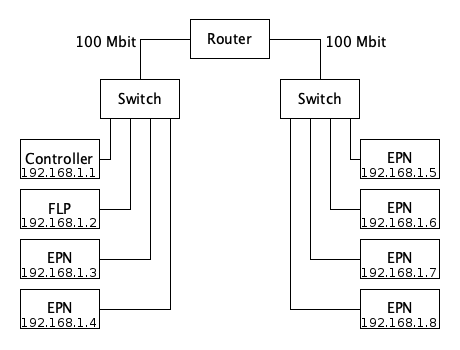
\includegraphics[width=0.45\textwidth]{images/network-primary-interface} & 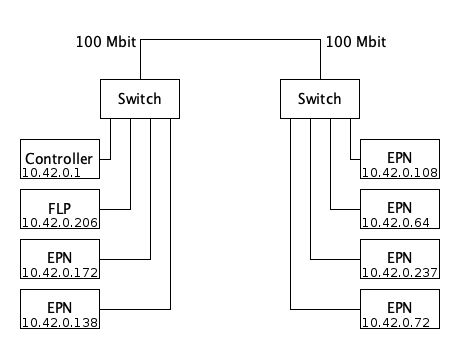
\includegraphics[width=0.45\textwidth]{images/network-auxiliary-interface} \\ \hline
		\end{tabular}
		\caption{Network interfaces that are available to nodes.}
		\label{tab:specs}
	\end{center}
\end{table}

\subsubsection{Results}
Losses across different configurations were there is one FLP in the network are extremely similar to the network throughput baseline experiment. This is likely due to the inability to cause out-of-order errors as there is only a single FLP in the network.

When introducing the second FLP into the network losses start to occur even at lower throughput than the synthetic benchmark.

\begin{table}[H]
	\textbf{Mean message loss - 1500 messages sent at an rate of 50hz (30 seconds)}	
	\begin{center}
		\begin{tabularx}{\textwidth}{ | X | X | X | X | X | }
			\hline
			\textbf{\#} & \textbf{Number of FLP’s} & \textbf{Message size (per FLP)} & \textbf{Mean loss (total)} & \textbf{Mean loss (\%)} \\ \hline
			
			1 & 1 & 232000 & 0 & 0.00 \\ \hline
			\underline{2} & \underline{1} & \underline{235000} & \underline{0} & \underline{0.00} \\ \hline
			3 & 1 & 238000 & 0 & 0.00 \\ \hline
			8 & 2 & 116000 & 7.44 & 0.50 \\ \hline
			\underline{9} & \underline{2} & \underline{117500} & \underline{5.11} & \underline{0.34}\\ \hline
			10 & 2 & 119000 & 11.11 & 0.74 \\ \hline
		\end{tabularx}
		\caption{Comparing loss of configurations with an 50Hz event rate.}
		\label{tab:specs}
	\end{center}
\end{table}

The losses with 2 FLP’s are higher with an event rate of 200Hz all of the losses were due to out-of-order errors directly  showing that the tighter timing constraints increase the amount of errors that occur at the same bandwidth.

\begin{table}[H]
	\textbf{Mean message loss - 6000 messages sent at an rate of 200hz (30 seconds)}	
	\begin{center}
		\begin{tabularx}{\textwidth}{ | X | X | X | X | X | }
			\hline
			\textbf{\#} & \textbf{Number of FLP’s} & \textbf{Message size (per FLP)} & \textbf{Mean loss (total)} & \textbf{Mean loss (\%)} \\ \hline
			
			4 & 1 & 58000 & 0 & 0.00 \\ \hline
			\underline{5} & \underline{1} & \underline{58750} & \underline{0} & \underline{0.00} \\ \hline
			6 & 1 & 59650 & 0 & 0.00 \\ \hline
			7 & 1 & 65000 & 441.89 & 7.35 \\ \hline
			11 & 2 & 29000 & 30.56 & 0.51 \\ \hline
			\underline{12} & \underline{2} & \underline{29375} & \underline{52.67} & \underline{0.87}\\ \hline
			13 & 2 & 29750 & 53.34 & 0.87 \\ \hline
			14 & 2 & 32500 & 85.56 & 1.42 \\ \hline
		\end{tabularx}
		\caption{Comparing loss of configurations with an 200Hz event rate.}
		\label{tab:specs}
	\end{center}
\end{table}

\subsection{Comparing long \& short runs}
Similar configurations should result in similar loss even if the duration is varied, on the condition that the duration of the test is sufficient to correctly measure the desired characteristics. The results from comparing short \& long runs, however, show that there is a measurable difference. The results highlighted in red have a higher long run percentage loss than the short run equivalent, while the results highlighted in green have a lower long run percentage loss over the short run.

\begin{table}[H]
	\textbf{Comparing losses of 30 second (short) \& 3 minute (long) runsw}	
	\begin{center}
		\begin{tabular}{ | l | l | l | l | }
			\hline
			\textbf{\#} & \textbf{Mean loss short-run (\%)} & \textbf{Mean loss long-run (\%)} \\ \hline
			
			1 & 0.00 & 0.00 \\ \hline
			2 & 0.00 & 0.00 \\ \hline
			\rowcolor{red}
			3 & 0.00 & 0.27 \\ \hline
			4 & 0.00 & 0.00 \\ \hline
			5 & 0.00 & 0.00 \\ \hline
			\rowcolor{red}
			6 & 0.00 & 1.23 \\ \hline
			\rowcolor{red}
			7 & 7.35 & 9.63 \\ \hline
			\rowcolor{green}
			8 & 0.50 & 0.00 \\ \hline
			\rowcolor{green}
			9 & 0.34 & 0.00 \\ \hline
			\rowcolor{green}
			10 & 0.74 & 0.01 \\ \hline
			\rowcolor{green}
			11 & 0.51 & 0.06 \\ \hline
			\rowcolor{green}
			12 & 0.88 & 0.01 \\ \hline
			\rowcolor{green}
			13 & 0.89 & 0.06 \\ \hline
			\rowcolor{green}
			14 & 1.39 & 0.21 \\ \hline
		\end{tabular}
		\caption{Effects of different iteration times on the percentage of loss during experiments.}
		\label{tab:specs}
	\end{center}
\end{table}

In all the green highlighted configurations there were 2 FLP’s in the network moreover all the losses were due to so called out-of-order errors. An out-of-order errors occurs when an EPN receives 2 messages from the FLP’s but each one with a different heartbeat, as a result the EPN invalidates the data and discards it so it can continue receiving new messages. Out-of-order errors are more likely to occur with tighter timing constraints or with fewer EPN’s in the network. The lower percentage loss on long runs might indicate that most of the out-of-order events occur during the beginning of the experiment and eventually settle out or at least become less likely to occur.

In all the red highlighted configurations the total size of accumulated messages multiplied by the rate of events exceeded the determined maximum throughput as determined in the synthetic benchmark. The results show that in the short run exceeded these network limits does not result in detected losses, however, in the long runs this does result in losses. This is likely due to network buffers which are temporarily capable of resolving the exceeded limits.


\section{Zookeeper throughput experiment}
The round-robin blacklist implementation using \hyperref[sec:ref12]{zookeeper [12]} has the following throughput:
\begin{itemize}
	\itemsep 0em
	\item Using packet size: 232000 bytes
	\item 2 flps - 5 epns - 60 tfps - measured input: 18 packets (3,67MB per epn = 18,8 MB/s total)
	\item 1 flps - 5 epns - 60 tfps - measured input: 12,5 packets (2,16 MB per epn = 10,8 MB/s total)
\end{itemize}

The implementation offers a robust system: the order of which flp/epn/icn startup or shutdown has no impact on the system. With a failover of any of the three nodes the system will continue working, after a reset the node will again be included in the system.

The blacklist algorithm has a different approach than the previous \hyperref[sec:ref13]{version [13]}. Instead of editing fairmq source code to allow for removing a channel from the channel list contained in MQProgOptions, compared to the new version that maintains a list of the online nodes so it is known which channels not to use. This allows for significant faster reinitializing of the node, since the channel doesn’t have to be broken down, instead the channels stays unused until the node comes back online in which case the node will be added to the list of online nodes. 

Multiple small improvements have been made, such as: no source-code editing of fairmq (so that is compatible to further versions), flp only retrieves zk values of new epns (not all), uses watchers, can detect restarted nodes, relieved network load by using direct channels from flp to icn (instead of using zookeeper), finally better naming and file structure in general.


\section{Results}
In this section the results from different experiments are compared as well as data from the synthetic benchmark. The information will be used to draw conclusion and recommend further work.

During the synthetic benchmark the network was able to sustain a throughput of 94Mbit while during the network baseline only 93Mbit could be achieved with an single FLP, however the network baseline only used the primary networking interface for all data and ran at an event rate of 200Hz. The additional results from the round robin ICN experiment show that the 94Mbit throughput can be sustained at both 50 \& 200Hz when using the auxiliary networking interface for communication between ICN to FLP and EPN to ICN.

\begin{center}
	\begin{figure}[H]
		\includegraphics[width=\textwidth]{"images/The effect on loss due to the unavailability of the auxiliary network interface"}
	\end{figure}
\end{center}

This sustained throughput of 94Mbit was only possible with a single FLP in the network while with 2 FLP’s there were still losses at 93Mbit throughput, although these losses were around 0.5\% for both 50 \& 200Hz event rates. The experiments show significant data that the 200Hz event rate could be sustained by an round robin algorithm with only a small reduction in network throughput.

\begin{center}
	\begin{figure}[H]
		\includegraphics[width=\textwidth]{"images/Effects of increased event rates on the loss for Round Robin with 2 FLP's"}
	\end{figure}
\end{center}

Finally the variation of iteration time from 30 seconds to 3 minutes has shown that this can have an effect of the loss that will be measured during the experiment. The total losses measured for both 30 second and 3 minute iterations are relatively low (always below 10\% and regularly below 3\%), however, the difference between the two iteration times can be as much as 650\%. This is an substantial difference that shows that other iteration times than 30 seconds should be considered in upcoming experiments.

\begin{center}
	\begin{figure}[H]
		\includegraphics[width=\textwidth]{"images/Effects of iteration time during round robin ICN experiment for 1 FLP"}
	\end{figure}
\end{center}

\begin{center}
	\begin{figure}[H]
		\includegraphics[width=\textwidth]{"images/Effects of iteration time during round robin ICN experiment for 2 FLP"}
	\end{figure}
\end{center}

\subsection{Metricbeat}
During the round robin ICN experiments metricbeat was used on the raspberry pi nodes to record metric data, unfortunately the results from this data proved unusable due to unreliability as well as the metricbeat process requiring a lot of system resources. The metricbeat process occasionally caused 65\% CPU utilization, additionally many graphs tended to be, making it hard to correlate them. Many of the nodes stopped correctly reporting metrics after a period of time which required the restarting of the metricbeat process to be resolved.

\begin{center}
	\begin{figure}[H]
		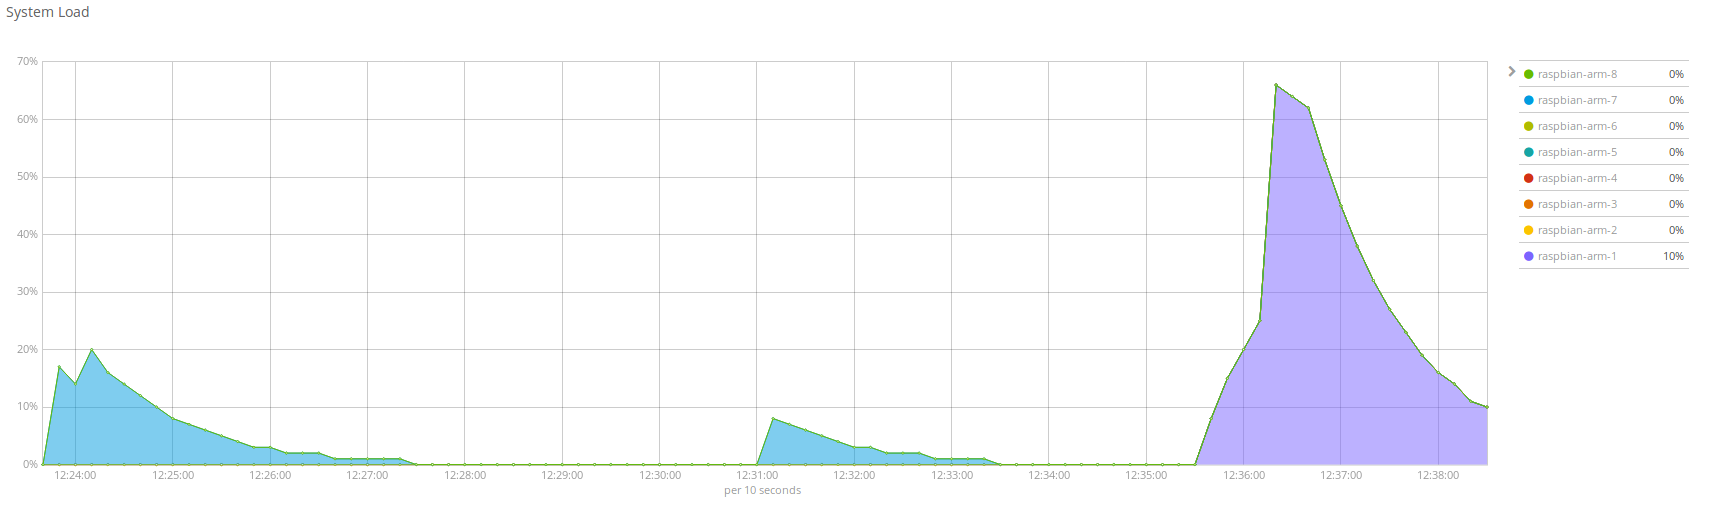
\includegraphics[width=\textwidth]{images/metric-load}
		\caption{Graph depicting the occasional 65\% CPU utilization which was determined to be metricbeat using tools as Htop.}
		\label{fig:ssh}
	\end{figure}
\end{center}


\section{Conclusion}
200Hz event rates should be manageable with only a small reduction in throughput when using the round robin algorithm, additional experiments with more nodes are required.

Metricbeat could be useful but it requires a lot of effort to be correctly configured in combination with Logstash, Elasticsearch \& Kibana. However, it might be unfeasible to run this service on ARM based nodes (such as Raspberry PIs) and additional work is required to determine if it is feasible.

Future experiments should take multiple iteration times into account as this parameter can affect results. Perhaps previous experiments should be repeated with different iteration times.


\section{Discussion}
Additional experiments with more nodes are required to better determine the effects of the round robin algorithm at 200Hz event rate. During this experiments, additional metrics would be of great value, but the overall feasibility of metricbeats and the entire MELK stack needs to be properly evaluated, especially for the ARM platform. In addition to the increased amount of nodes a larger variety of iteration times could also benefit the results.


\begin{thebibliography}{}
	\label{sec:ref01}\bibitem{}\href{https://github.com/hexoxide/O2-Balancer}{O2-Balancer}
	\label{sec:ref02}\bibitem{}\href{https://github.com/valvy/BalancerScripts}{Balancer Scripts}
	\label{sec:ref03}\bibitem{}\href{http://cds.cern.ch/record/2011297/files/ALICE-TDR-019.pdf?version=3}{ALICE Technical Design Report}
	\label{sec:ref04}\bibitem{}\href{https://iperf.fr/}{iPerf}
	\label{sec:ref05}\bibitem{}\href{https://github.com/hexoxide/documentation/blob/master/draw-io/Network-Primary-Auxillary-Dec-14.png}{Networking diagram with auxiliary interface}
	\label{sec:ref06}\bibitem{}\href{https://github.com/hexoxide/raspberry-dependency}{Raspberry Dependency}
	\label{sec:ref07}\bibitem{}\href{https://github.com/hexoxide/BalancerScripts2}{Balancer Scripts 2}
	\label{sec:ref08}\bibitem{}\href{https://github.com/hexoxide/O2-Balancer2}{O2-Balancer 2}
	\label{sec:ref09}\bibitem{}\href{https://github.com/hexoxide/documentation}{Documentation}	
	\label{sec:ref10}\bibitem{}\href{https://github.com/hexoxide/O2-Balancer2/commits/experiment-1}{O2-Balancer 2 Commits}
	\label{sec:ref11}\bibitem{}\href{https://github.com/hexoxide/documentation/tree/cdbb643c6ebc875e73e8c1c2433c6d14cda05aca}{Documentation cdbb643}
	\label{sec:ref12}\bibitem{}\href{https://github.com/hexoxide/O2-Balancer2/tree/zookeepertje}{O2-Balancer 2 Zookeepertje}
	\label{sec:ref13}\bibitem{}\href{https://github.com/valvy/}{GitHub Valvy Profile}
\end{thebibliography}


\section{Appendix}

\subsection{Commands to replicate network throughput baseline}
\label{sec:appendix01}
XXXXXX = Message size \\
YYY = Number of FLP’s in the network

\subsubsection{Commands for experiment with single network card}
\begin{lstlisting}
./icn/icn --severity trace --verbosity high --id 1 --iterations 6000 --rate 200 --channel-config name=broadcast,type=pub,method=bind,rateLogging=0,address=tcp://*:5005 name=feedback,type=pull,method=bind,rateLogging=0,address=tcp://*:5000
\end{lstlisting}

\begin{lstlisting}
./flp/flp --severity trace --verbosity high --id 1 --bytes-per-message XXXXXX --channel-config name=broadcast,type=sub,method=connect,rateLogging=1,address=tcp://192.168.1.4:5005
\end{lstlisting}

\begin{lstlisting}
./epn/epn --severity trace --verbosity high --id 1 --num-flp YYY --channel-config name=1,type=pull,method=bind,address=tcp://*:5555,rateLogging=1 name=feedback,type=push,method=connect,address=tcp://192.168.1.4:5000
\end{lstlisting}

\subsubsection{Commands for experiment with dual network cards}
\begin{lstlisting}
./icn/icn --severity trace --verbosity high --id 1 --iterations 6000 --rate 200 --channel-config name=broadcast,type=pub,method=bind,rateLogging=0,address=tcp://*:5005 name=feedback,type=pull,method=bind,rateLogging=0,address=tcp://*:5000
\end{lstlisting}

\begin{lstlisting}
./flp/flp --severity trace --verbosity high --id 1 --bytes-per-message XXXXXX --channel-config name=broadcast,type=sub,method=connect,rateLogging=1,address=tcp://10.42.0.138:5005
\end{lstlisting}

\begin{lstlisting}
./epn/epn --severity trace --verbosity high --id 1 --num-flp YYY --channel-config name=1,type=pull,method=bind,address=tcp://*:5555,rateLogging=1 name=feedback,type=push,method=connect,address=tcp://10.42.0.138:5000
\end{lstlisting}

\subsection{Commands to replicate round robin}
\label{sec:appendix02}
XXXXXX = Message size \\
YYY = Rate of the experiment \\
ZZZ = Number of iterations \\
WWW = EPN number

\subsubsection{Build configuration}
\begin{lstlisting}
cmake -DCMAKE_BUILD_TYPE=Release -DENABLE_DOXY=false ..
make 
make test
\end{lstlisting}

\subsubsection{1 FLP}
\begin{lstlisting}
./icn/icn --control static --severity trace --verbosity high --id 1 --iterations ZZZ --rate YYY --channel-config name=broadcast,type=pub,method=bind,rateLogging=1,address=tcp://*:5005 name=feedback,type=pull,method=bind,rateLogging=1,address=tcp://*:5000
\end{lstlisting}

\begin{lstlisting}
./flp/flp --severity trace --verbosity high --id 1 --bytes-per-message XXXXXX --channel-config name=broadcast,type=sub,method=connect,rateLogging=1,address=tcp://10.42.0.1:5005
\end{lstlisting}

\begin{lstlisting}
./epn/epn --control static --severity trace --verbosity high --id WWW --primary-interface eth0 --num-flp 1 --channel-config name=WWW,type=pull,method=bind,address=tcp://*:5555,rateLogging=1 name=feedback,type=push,method=connect,address=tcp://10.42.0.1:5000
\end{lstlisting}

\subsubsection{2 FLP}
\begin{lstlisting}
./icn/icn --control static --severity trace --verbosity high --id 1 --iterations ZZZ --rate YYY --channel-config name=broadcast,type=pub,method=bind,rateLogging=1,address=tcp://*:5005 name=feedback,type=pull,method=bind,rateLogging=1,address=tcp://*:5000
\end{lstlisting}

\begin{lstlisting}
./flp/flp --severity trace --verbosity high --id 1 --bytes-per-message XXXXXX --channel-config name=broadcast,type=sub,method=connect,rateLogging=1,address=tcp://10.42.0.1:5005
\end{lstlisting}

\begin{lstlisting}
./epn/epn --control static --severity trace --verbosity high --id WWW --primary-interface eth0 --num-flp 2 --channel-config name=WWW,type=pull,method=bind,address=tcp://*:5555,rateLogging=1 name=feedback,type=push,method=connect,address=tcp://10.42.0.1:5000
\end{lstlisting}


\end{document}
